\section{牛顿第一运动定律}\label{sec:3-6}

我们已经知道,机械运动是多种多样的。
有一个很重要的问题非常值得研究,这就是为什么有的物体保持静止,有的物体又在运动?
为什么有的物体做直线运动,有的物体又做曲线运动?
为什么有的物体做匀速运动,有的物体又做变速运动?
一句话,物体做各种运动的原因是什么呢?我们将在这几节里初步探讨一下这个问题。

人们很早就关心这个重要的问题。
两千多年前,古希腊哲学家亚里士多德(公元前 384 ~ 322)认为,必须有力作用在物体上,
物体才能运动,没有力的作用,物体就要静止下来。他的说法跟人们的某些日常经验相符。
譬如,用力推桌子,桌子就运动起来,停止用力,桌子就停下来。
因此,亚里士多德的说法在差不多两千年里一直得到人们的公认。

但是,随着科学的发展,亚里士多德的这个被沿用了近两千年的说法,终于在 17 世纪被伽利略证明不是正确的。

为了理解伽利略的研究,让我们先做一个简单的实验。用力推一辆小车,使它动起来。
停止用力后,小车并不马上停止,还要前进一段距离才停下来。
没有力推它了,小车还能运动,亚里士多德的说法不能解释这个现象。
我们再在三种不同的表面上做这个实验(图 \ref{fig:3-5}),一种是铺了毛巾的毛糙表面,
一种是铺了棉布的不太光滑的表面,一种是光滑的木板表面。
每次实验都用同一个小车,从同样高的斜面上滑下来,使它在三种表面上开始运动时的速度相伺。
从实验可以看出,在光滑的木板上前进的距离最长,在棉布的表面上前进的距离较短,在毛巾表面上前进的距离最短。
我们知道,小车在这些表面上运动时是要受到阻力的,木板对小车的阻力最小,棉布对小车的阻力较大,毛巾对小车的阻力更大。
可见,在越光滑的表面上,小车受到的阻力越小,它就走得越远,它的运动就越接近匀速运动。

\begin{figure}[htbp]
    \centering
    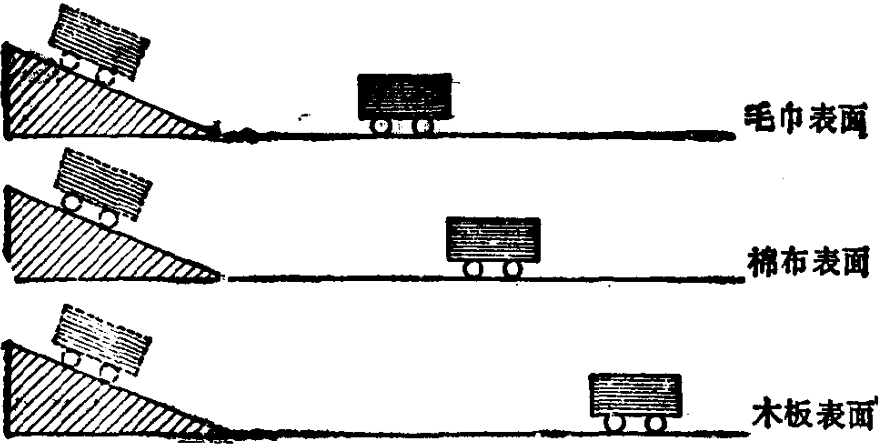
\includegraphics[width=0.6\textwidth]{../pic/czwl1-ch3-5}
    \caption{}\label{fig:3-5}
\end{figure}

伽利略研究了类似的现象,并且进一步提出了一个重要的问题。
如果运动物体不受到任何力的作用,又会怎样呢?
他对这个问题进行了实验研究和深入的思考,最后得到这样的结论:
\CJKunderwave{如果物体在运动中不受任何力的作用,它的速度将保持不变,永远运动下去}。

后来,别的科学家又进一步发展了伽利略的思想,
指出\CJKunderwave{如果运动物体不受任何力的作用,它既不会向右偏,也不会向左偏,将永远沿直线运动下去}。

英国科学家牛顿概括了伽利略等人的研究成果,总结出如下的规律。

\textbf{一切物体在没有受到外力作用的时候,总保持匀速直线运动状态或静止状态}。

这就是著名的\textbf{牛顿第一运动定律}。


\nonumsection{阅读材料:牛顿}

\begin{wrapfigure}[9]{r}{4cm}
    \centering
    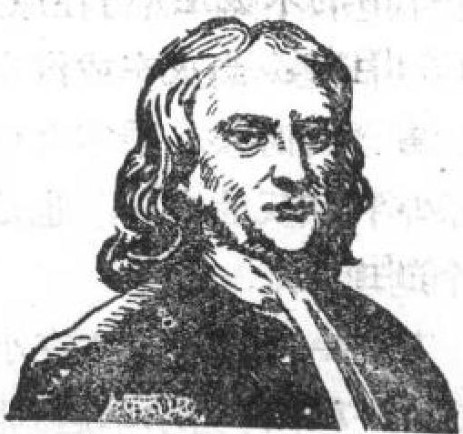
\includegraphics[width=4cm]{../pic/czwl1-ch3-newton}
    \caption*{牛顿(1642 ~ 1727)}
\end{wrapfigure}

牛顿生于 1642 年。他是人类历史上最著名的最伟大的科学家之一。他在科学上作出了许多重大的发现。
他发现的包括我们刚刚学过的定律在内的关于运动的三个定律,是整个力学的基础。
他还发现了万有引力定律,白光分解为种色光的现象。此外,他在数学领域中还有许多重大发现。
牛顿虽然作出了这么多重大的贡献,但他却是很谦虚的,他曾经锐过:“我不知道世人对我是怎样看的,
不过我只觉得自己好象是一个在海滨玩耍的孩子,有幸拾到光滑美丽的石子,但真理的大海,我还是没有发现。”
“我所以有这样的成就,是因为我站在巨人们的肩膀上的缘故。”


